\begin{surferIntroPage}{Weltrekordflächen}{record_chmutovoktic}{Weltrekord-Flächen}
    Eine Fläche heißt \emph{nicht-singulär} oder \emph{glatt}, wenn sie keine spitzen Stellen oder Selbstdurchdringungen (\emph{Singularitäten} genannt) hat, z.B.\ eine Kugel oder ein Torus, siehe Abbildung. 
    Dies ist so gut wie immer der Fall, wenn wir die
    Fläche zufällig wählen. 
    \begin{center}
      \vspace{-0.2cm}
      \begin{tabular}{@{}c@{}c@{}c@{\quad}c@{}c@{}c@{}c@{}}
        \begin{tabular}{@{}c@{}}
          glatt:
        \end{tabular}
        &
        \begin{tabular}{@{}c@{}}
          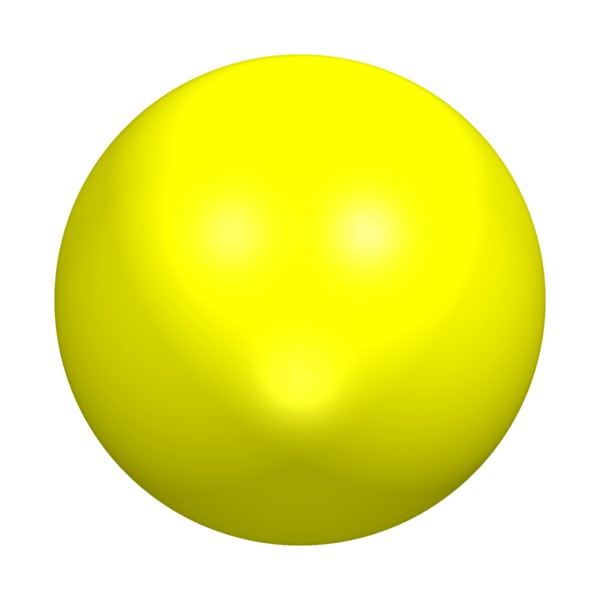
\includegraphics[width=1.1cm]{./../../common/images/kugel}
        \end{tabular}
        &
        \begin{tabular}{@{}c@{}}
          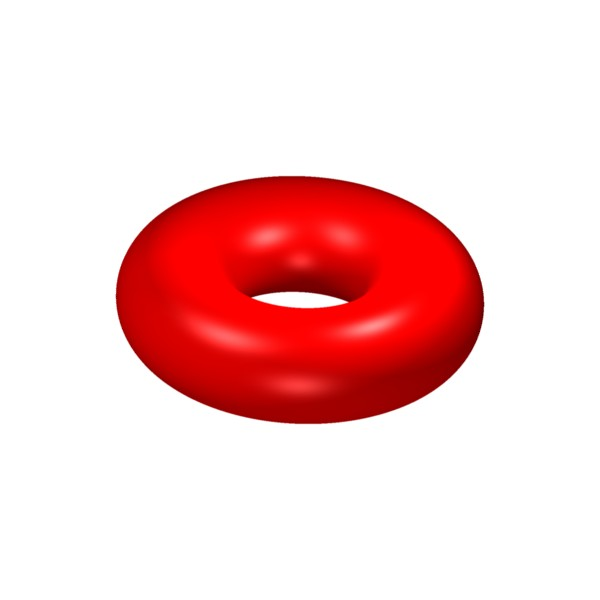
\includegraphics[width=1.1cm]{./../../common/images/torus}
        \end{tabular}
        &
        \begin{tabular}{@{}c@{}}
          viele\\
          Singularitäten:
        \end{tabular}
        &
        \begin{tabular}{c@{}@{}}
          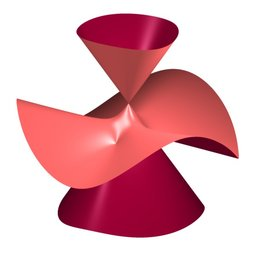
\includegraphics[width=1.1cm]{./../../common/images/cayley}
        \end{tabular}
        &
        \begin{tabular}{c@{}@{}}
          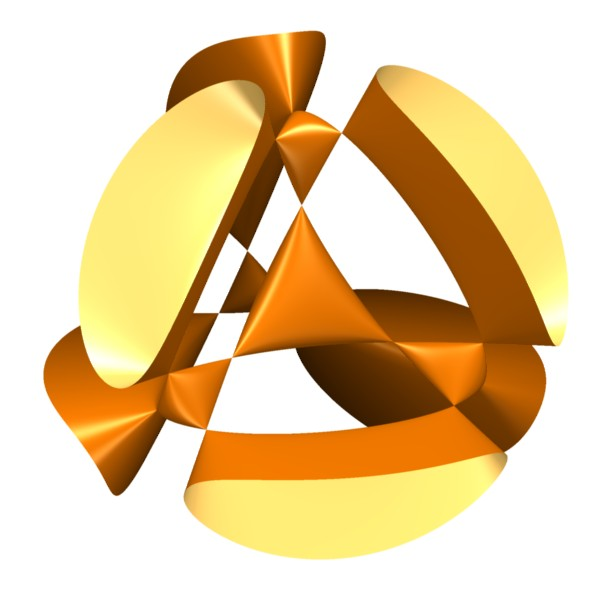
\includegraphics[width=1.1cm]{./../../common/images/kummer}
        \end{tabular}
        &
        \begin{tabular}{c@{}@{}}
          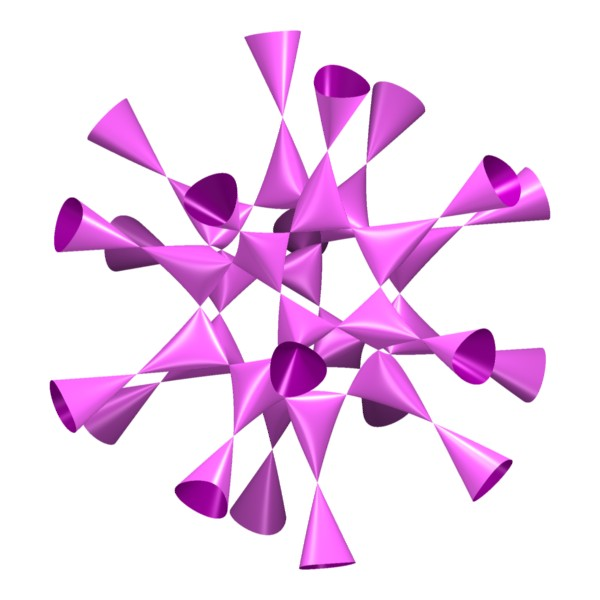
\includegraphics[width=1.1cm]{./../../common/images/barth_sextic}
        \end{tabular}
      \end{tabular}
    \end{center}
    \vspace{-0.2cm}
    Nur spezielle Flächen weisen Singularitäten auf. Das macht diese Singularitäten zu den interessantesten Punkten der Fläche. 
    Alle Flächen im SURFER bestehen aus den Nullstellen von Polynomen. Das bedeutet, dass die Variablen in den Formeln nur ganzzahlige positive Exponenten haben. Den höchsten Exponenten des Polynoms bezeichnet man auch als \emph{Grad} des Polynoms. 
    In der Mathematik lautet eine Frage in der Forschung wie viele Singularitäten eine Fläche mit einem bestimmten Grad haben kann. 
    Den Grad eines Polynoms bezeichnen wir mit $d$ und die Anzahl der Singularitäten mit $\mu(d)$. Diese Zahl $\mu(d)$ ist sehr schwer zu ermitteln. Für kleine Exponenten wie $d=1,2,3,4$ ist sie seit dem 19.\ Jahrhundert bekannt, doch für
    $d=5$ wurde die Zahl erst 1980 und für $d=6$ sogar erst 1996 herausgefunden.
    Für ein Polynom vom Grad $7$ ist die maximale Anzahl der Singularitäten bislang unbekannt. Es gibt jedoch schon einige Untersuchungen dazu.
    Eine endgültige Beantwortung der Frage für beliebiges $d$  liegt also noch in weiter Ferne.
    Einige bisher bekannte Werte:
    \begin{center}
      \begin{tabular}{r|cccccccc|c}
        $d$ & $1$ & $2$ & $3$ & $4$ & $5$ & $6$ & $7$ & $8$ & $d$\\
        \hline
        \hline
        \rule{0pt}{1.2em}$\mu(d)\ge$ & $0$ & $1$ & $4$ & $16$ & $31$ & $65$ &
        $99$ & $168$ & 
        $\approx \frac{5}{12}d^3$\\[0.3em]
        \hline
        \rule{0pt}{1.2em}$\mu(d)\le$ & $0$ & $1$ & $4$ & $16$ & $31$ & $65$ &
        $104$ & $174$ & $\approx \frac{4}{9}d^3$
      \end{tabular}
    \end{center}
\end{surferIntroPage}
